%
\begin{isabellebody}%
\setisabellecontext{thesis{\isacharunderscore}{\isadigit{5}}{\isacharunderscore}discussion}%
%
\isadelimtheory
%
\endisadelimtheory
%
\isatagtheory
%
\endisatagtheory
{\isafoldtheory}%
%
\isadelimtheory
%
\endisadelimtheory
%
\isadelimdocument
%
\endisadelimdocument
%
\isatagdocument
%
\isamarkupsection{Discussion\label{discussion}%
}
\isamarkuptrue%
%
\isamarkupsubsection{Automated Moral Agents in Practice \label{AIethics}%
}
\isamarkuptrue%
%
\endisatagdocument
{\isafolddocument}%
%
\isadelimdocument
%
\endisadelimdocument
%
\begin{center}
\begin{figure}
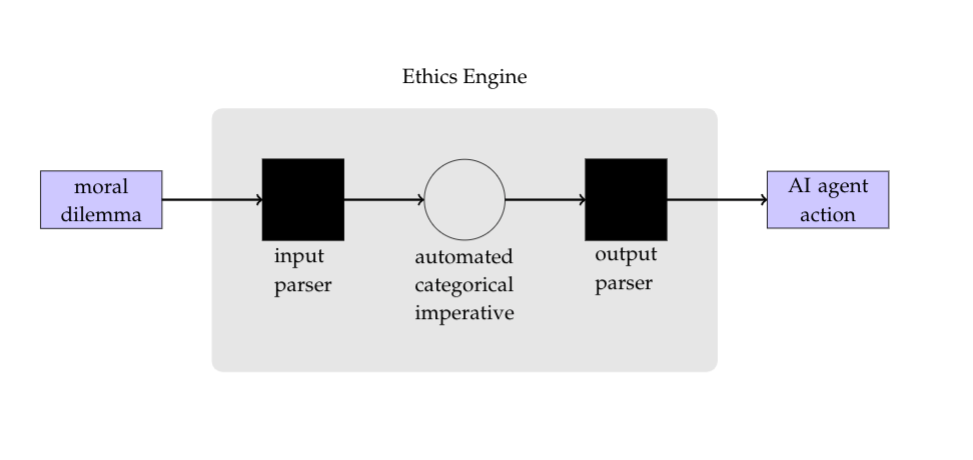
\includegraphics[scale=0.43]{AI_engine.png}
\caption{An example of an ethics engine for an artificial agent. This ethics engine passes a moral dilemma 
through an input parser, applies the automated categorical imperative test, and finally processes the 
output using an output parser, producing a prescription for action. I contribute the automated categorical 
imperative component.} \label{fig:AIengine}
\end{figure}
\end{center}
%
\begin{isamarkuptext}%
In Chapter \ref{applications}, I demonstrated that my system is capable of performing sophisticated,
nuanced ethical reasoning. In this section, I outline the additional components necessary for my system
to guide AI agents in practice. As it stands, my system is a categorical imperative library that, given
sufficient factual or ``common sense'' background, can take 
as input the logical representation of a maxim and return its moral status (if it is obligatory, 
prohibited, or permissible). My project potentially 
serves as one component of an ``ethics engine'' that an AI agent could use to make ethical decisions.
For example, my system could be combined with an input parser to translate moral dilemmas as represented 
to the AI agent into maxims in my logic. An output parser could translate my system's output
into a prescription for action that the AI agent could act on. Figure \ref{fig:AIengine} depicts the 
workflow of this example ethics engine.

In this workflow, an AI agent is faced with a moral dilemma in some internal representation. The input
parser translates this internal representation into an appropriate logical representation, i.e. 
a circumstance, act, goal tuple. The output parser translates the output of the categorical imperative
library (the moral status of the maxim as obligatory, prohibited, or permissible) to a prescription for
action. In order for my system to be used in an AI agent using the workflow
above, future work must develop such input and output parsers.

One of the biggest challenges for an ethics engine is the development of an input parser. An input parser 
for my implementation of automated Kantian ethics must translate a complex real-world situation into a flat, logical representation.
This requires that the input parser determine which circumstances are morally relevant
to a maxim, a controversial judgement. As mentioned in Section \ref{whatisamaxim},
there is robust debate on the circumstances that should be considered when formulating a maxim, 
inspired by a common criticism of Kantian ethics called the tailoring objection. Recall that the 
tailoring objection is the worry that arbitrarily specific 
circumstances render any maxim universalizable. For example, consider the maxim ``When my name is Lavanya Singh 
and I am wearing a purple shirt and it is November 26th, I will lie in order to get some easy cash.'' 
Even if this maxim is willed universally, the circumstances are so 
specific that lying will not become the general mechanism for getting easy cash, so the lender will 
believe my lie and the maxim will remain effective. By tailoring the circumstances, any maxim can 
evade universalization.

The Kantian response to this criticism is to require that the circumstances included in the formulation
of the maxim be morally relevant. In the example above, my purple shirt and the date have no bearing on 
the moral status of lying. On the other hand, consider the maxim, ``When I am unemployed, I will murder
someone in order to take their job.'' The circumstances of being unemployed clearly have some bearing on the moral
relevance of the murder in question; they speak to the motivation for the murder. 

While this view has intuitive appeal, it raises the question of how we can determine
which circumstances are morally relevant. O'Neill answers this question by noting that the Formula of Universal Law is 
a ``test of moral worth rather than of outward rightness'' \citep[98]{constofreason}. The FUL is a way 
for an agent to decide how they should behave, not for a third-party to judge their behavior. Ethics is 
a personal process and the FUL is designed to help agents make decisions for themselves. Because agents use 
the FUL to evaluate their own behavior, the test is at its 
best when they make a good faith effort to isolate the \emph{principle} of their action, rather than some
``surface intent'' \citep[87]{constofreason}. The FUL is supposed to determine if an agent's principle of action
is universally consistent, so it is most effective when an agent accurately formulates the principle that
they act on. Circumstances are morally relevant if they reflect the way that the agent is 
thinking about their own action. In the example above, the circumstance of wearing a purple shirt doesn't reflect
the principle of the liar's action. Its inclusion is a disingenous attempt to evade the universalizability
test, but because the FUL is a test of personal integrity, it cannot withstand this kind of mental
gymnastics. 
 
While the above account explains how a well-intentioned human agent can determine 
morally relevant circumstances, the challenge remains open for automated ethics. However an action is turned into a maxim for my system 
to process, whether manually as I did in Chapter \ref{applications} or using an automatic input 
parser, this transformation must be a good-faith attempt to capture the principle of action. 
Correctly formulating a maxim requires what Kantians call ``practical judgement,'' or
common sense reasoning and factual background \citep{oneilluniversallaws}. Returning to the example above, noticing that being 
unemployed may contribute to one's desire to steal another's job requires practical
judgement, not just pure reason alone. Translating everyday situations into appropriate maxims is
the bulk of the reasoning that a Kantian human being does when making decisions. Automating this
reasoning requires endowing a machine with common sense. 

The challenge of formulating a maxim is one of the biggest obstacles to using my categorical imperative library
in an AI ethics engine. One solution is for a human being to perform the role of the input
parser by supervising the operation of an AI agent. When the agent stumbles onto
an ethical dilemma, the human could take over, formulate
the right question, and feed it into the categorical imperative library to see what action the categorical 
imperative would prescribe. Alternatively, AI developers can identify expected ethical dilemmas 
that the machine may face in advance and hardcode their own judgements for these dilemmas. 
For proponents of the ``human-in-the-loop'' model of AI ethics, in which
ethical AI requires that humans guide machines, this kind of human involvement may be a feature \citep{loop}.
Both of these solutions imply that the outcome of the universalizability test will depend on how the 
human formulates the maxim; if the human puts garbage into the test, the test will return garbage out.

It is likely that, regardless of the strengths of the human-in-the-loop model, fully automated AI 
agents will exist. Even if developing this kind of AI is irresponsible,
such developments are likely and will require ethics engines, or risk no consideration of ethics at all.
In such a world, the input parser in my ethics engine would have to be automated.
It is likely that, just as implementations of automated ethics choose 
a particular ethical theory and implement it, different implementations of such an input parser may 
adopt different interpretations of maxim formulation and morally relevant circumstances. 

These interpretations could inspire heuristics to classify circumstances as morally 
relevant. For example, one such attempt could define a moral closeness relation between an action, a 
goal, and circumstances. This heuristic could define morally relevant circumstances as those that 
reach a certain closeness threshhold with the action and the goal. Another possible heuristic could 
define some set of morally important entities, and classify morally relevant circumstances as those
that involve morally important entities. I discuss a potential machine-learning based approach which formulates
maxims based on a training set of appropriately formulated maxims in Section \ref{amapossible}. This 
approach mimics how human beings formulate maxims; we use common sense and prior situational, 
factual, and ethical knowledge to isolate our principle of action. Determining morally relevant circumstances, 
either using heuristics or human involvement, is a ripe area for future work.

Once the input has been parsed, either by a human or a machine, into a sentence in my logic, my 
project can evaluate its moral status using my implementation of 
the FUL. Concretely, my project returns a value indicating if the maxim is obligatory, permissible, 
or prohibited. The maxim is prohibited if it fails the universalizability test, permissible if it passes, and obligatory 
if its negation fails the universalizability test. All three of these properties require testing if a 
certain theorem holds or not in my logic, a calculation that I demonstrate in Section \ref{testing}. 
Testing these properties requires that my system have a database of common sense or factual background. 
Different applications of my system may require different factual background (e.g. a self-driving car 
needs to know traffic regulations), so this common sense database will need to be application 
specific. As demonstrated in the examples in Chapter \ref{applications}, my system can produce sophisticated 
judgements with relatively little situational context. Thus, while my automated categorical imperative
requires some common sense and factual background, Chapter \ref{applications} demonstrates that automating
this common sense is less daunting than it seems.

My system's output could be converted into some actionable, useful response with an output parser, 
and then passed back to the AI agent. For example, if the AI agent is equipped to evaluate natural 
language prescriptions, the status of the maxim could be parsed into a natural language sentence. The 
input parser, categorical imperative, and output parser together constitute an ``ethics engine'' 
that AI developers could use in a variety of AI systems.

The ethics engine depicted above is a high-level example of one way to use my project to guide an artifical agent,
with additional work to parse the input and output of my implementation of the categorical imperative.
Effectively, the kind of automated ethics I implement could be part of a library that AI developers use to 
give AI agents the capacity for sophisticated ethical reasoning faithful to philosophical literature. 
This represents an improvement over existing automated ethics, which rarely captures the complexity 
of any ethical theory that philosophers plausibly defend.%
\end{isamarkuptext}\isamarkuptrue%
%
\isadelimdocument
%
\endisadelimdocument
%
\isatagdocument
%
\isamarkupsubsection{Computational Ethics \label{computationalethics}%
}
\isamarkuptrue%
%
\endisatagdocument
{\isafolddocument}%
%
\isadelimdocument
%
\endisadelimdocument
%
\begin{isamarkuptext}%
In addition to guiding AI agents, automated ethics can also help human beings make philosophical
progress. Just as theorem provers make mathematics more efficient and push mathematicians to think 
precisely about the phenomena they model, computational ethics can help philosophers ask and answer
new philosophical questions. In Section \ref{joking}, I presented one example of the power of computational ethics
by using my system to isolate a necessary and sufficient condition for the act of lying, or knowingly saying
something false, to be wrong. In this section, I share another example of the kind of philosophical 
insight that computational ethics can prompt and analyze the value that this tool can offer to philosophers.\footnote{
I present a final example of computational ethics in Appendix \ref{weirdtests}, where I resolve an ambiguity 
in Korsgaard's argument for the wrongness of false promising using my system \citep{KorsgaardFUL}.} 
Fields from protein folding to game theory are uncovering new insights using computational tools, and computational
ethics harnesses this power to inspire similar progress in philosophy.%
\end{isamarkuptext}\isamarkuptrue%
%
\isadelimdocument
%
\endisadelimdocument
%
\isatagdocument
%
\isamarkupsubsubsection{Example of a Philosophical Insight: Well-Formed Maxims%
}
\isamarkuptrue%
%
\endisatagdocument
{\isafolddocument}%
%
\isadelimdocument
%
\endisadelimdocument
%
\begin{isamarkuptext}%
As presented in Section \ref{formalizingful}, in the process of developing my formalization of
the FUL, I discovered that certain kinds of maxims are badly formed, or inappropriate inputs to the 
universalizability test. The FUL is consistent only if it holds for ``well-formed maxims,''
such that neither the act nor goal are already achieved in the given circumstances. Precisely, 
a circumstance, act, goal tuple (c, a, g) is well-formed if $(\neg (c \longrightarrow a) ) \wedge 
(\neg(c \longrightarrow g))$, or if the circumstances do not imply the act or the goal. The insight
that the FUL does not apply to badly-formed maxims has philosophical value and serves as evidence 
of the potential of computational ethics. In the next section, I explain and explore this insight using 
Kantian literature. In the following section, I demonstrate the philosophical implications of well-formed
maxims by using this insight to resolve a tension between self-doubt and self-respect. The idea of well-formed
maxims can guide the formulation of maxims and thus may have implications for many parts of Kantian ethics.

\noindent \textbf{Badly-Formed Maxims and Kantian Ethics}

Isabelle gave a logical argument for why the FUL can only hold for well-formed maxims, and I return to Kantian
literature to better understand this idea. In this section, I argue that 
because badly-formed maxims
neither change an agent's behavior nor generate meaningful obligations, they are not the right kinds of 
actions for practical reasoners to make moral judgements about. They cannot be action-guiding and are thus not the kind of problem that 
ethics should be concerned with. Moreover, under the Kantian account of the will, the very act of asking 
if a badly-formed maxim is prohibited generates a contradiction by undermining the will's authority over itself. 

Consider the example badly-formed maxim, ``When eating breakfast, I will eat breakfast in order to 
eat breakfast.'' There is something empty about this maxim because acting on it could never result in 
any action. If I adopt this maxim as a principle to live by,
I decide that, in the circumstances ``eating breakfast'' I will perform the act ``eating breakfast''
for the purpose ``eating breakfast.'' In these circumstances, the act has 
already been performed. Adopting this maxim as a law to live by does not change how I live. If I adopt 
this maxim, then when I am eating breakfast, I eat breakfast, but this statement is already tautologically true. 

Not only does a badly-formed maxim fail to prescribe action, any obligations or prohibitions it 
generates have already been fulfilled or violated. If a badly-formed maxim generates a prohibition, 
then this prohibition is impossible to obey, which is why my original version of the FUL was inconsistent. 
It is impossible to not eat breakfast while eating breakfast, because the circumstances assume that the 
act has happened. On the other hand, if a badly-formed maxim generates an obligation, then the obligation 
will have already been fulfilled. If you are required to eat breakfast while eating breakfast, then you've 
already fulfilled your obligation because the circumstances assume that the act has happened. Thus, 
a badly-formed maxim does not actually guide action because it doesn't generate new obligations or 
prohibitions. 

Because badly-formed maxims can't prescribe or alter action, they are not practically action-guiding and 
thus are not the right kinds of maxims for practical reasoners to evaluate. Insofar as ethics 
is supposed to guide action, badly-formed maxims cannot be part of this project because they
have no bearing on what someone should do. Practical reason is the kind of reason that helps us decide 
what we should do. A practical reasoner asks moral questions not as a mental puzzle or out of curiosity, but 
to decide how to act. A badly-formed maxim is not the kind of maxim that a practical reasoner should consider, because it
will have no bearing on what the agent should do.

Kantians can make an even stronger claim about badly-formed maxims—because maxims are laws that you 
give to yourself, asking if you should will a maxim as you will it undermines your will's law-giving 
ability. The circumstances of a badly-formed maxim assume that the agent has willed the maxim. Under 
the Kantian acount of willing, willing a maxim is equivalent to giving the maxim to yourself as a law. 
When you will a maxim, you commit yourself to the maxim's end. You cannot simultaneously 
commit yourself to a maxim and ask if you should be committing to it. To will the maxim is to adopt it as 
law—so the question, ``should I be willing this?'' is paradoxical. Either you haven't actually made 
the maxim your law (and thus haven't yet committed to it), or you aren't actually asking 
the question (because the decision has already been made). Because a maxim is a law that you give to 
yourself, you cannot question it absent a sufficient reason, such as a change in the circumstances. 
To question a law arbitrarily is to not regard it as a law at all. This kind of questioning amounts to 
questioning the will's authority over itself, but this is impossible. The will definitionally has authority 
over itself, for that is what it is to be a will. 

A skeptic may argue that we do often ask ``should I be doing this?'' as we do something. 
Can this kind of question ever be valid? To understand this worry, I consider the maxim, 
``When dancing, I should just dance for the sake of dancing.'' While this maxim appears to be badly-formed (the 
circumstance ``dancing'' implies the act and goal of dancing), it is a question that practical reasoners 
do ask. I argue that the correct interpretation of this maxim is no longer a badly-formed maxim.

Under one reading of this maxim, ``I should just dance'' is referring to a different act than the 
circumstance ``when dancing.'' The circumstance ``when dancing'' refers 
to rythmically moving your body to music, but ``I should just dance'' refers to dancing without anxiety, 
completely focused on the joy of dancing itself. More precisely, this maxim should read ``When 
dancing, I should abandon my anxiety and focus on dancing for the sake of dancing.'' This maxim when so 
modified is not badly-formed at all—abandoning anxiety and focusing on dancing is an entirely different act 
from moving your body rythmically to music. The circumstances do not entail the act or the goal because 
they refer to different meanings of the word dancing. Any valid reading of this maxim will have the structure above, 
in which the act is actually different from the circumstances. A reasoner cannot accept their will 
as law-giving, or commit themselves to an act, and simultaneously question the act. Either they must be 
questioning a different act or they must have recieved new information to prompt the questioning, 
modifying the circumstances of the original maxim. 

Another related worry concerns maxims that we think are prohibited. Consider the maxim modified to 
read ``When dancing and seeing a child drowning, I should dance for the sake of dancing.'' Clearly this 
maxim is fit for moral evaluation, and we expect a moral theory to prohibit this maxim. The circumstances 
``When dancing and seeing a child drowning'' appear to entail the act of dancing, and the maxim thus 
appears badly-formed. Once again, this maxim is formulated incorrectly. In this case, the question 
that the agent is actually asking themselves is ``should I continue dancing?'' That is the 
maxim that they will adopt or reject. They want to know if they should stop dancing and go help the child. 
Dancing at the current moment and dancing at the next moment are different acts, and the circumstances 
imply the former but not the latter. A badly-formed maxim would have circumstances and act both 
``dancing at moment t,'' but this maxim has circumstances ``dancing at moment t'' and act ``dancing 
at moment t+1.''

\noindent \textbf{Implications for Self-Doubt and Self-Respect}

Above, I defined badly formed maxims, a philosophical concept that I discovered
using computational ethics. In this section, I explore the implications of this concept for the ethical
tension between self-doubt and self-respect to show that computational ethics can result in insights with real 
philosophical weight. The debate between self-doubt and self-respect originates in epistemology, which 
values doubting your beliefs but also rationally requires that you believe that you are not mistaken 
(else you should update your beliefs). I present a parallel tension between self-doubt and self-respect
in ethics, where questioning your judgements is valuable but 
questioning a commitment as you make it is impossible. Ethical self-doubt and self-respect appear 
irresolvably opposed until they are understood through the lens of badly formed maxims. I argue that naive
conceptions of self-doubt are badly formed maxims in disguise. If we reformulate these maxims to be well-formed,
the tension between self-doubt and self-respect dissolves. I sketch the details of this argument in 
the rest of this section. I first introduce the tension between self-doubt and self-respect 
in epistemology, then explain the parallel tension in ethics, and finally present a resolution of this 
tension using badly-formed maxims. I conclude that well-formed maxims form a boundary condition for
the formulation of maxims, so they may resolve many debates in Kantian literature and ethics more generally.

In epistemology, there is a tension between the rational requirement to believe in yourself and the 
value of self-doubt, in moderation. Christensen presents the ``principle of self-respect,'' which requires 
that a rational agent refrain from believing that they have mistaken beliefs \cite[4]{christensen}. For example, I cannot 
rationally believe both that the sky is blue and that I believe that the sky is green. In other words, I cannot 
disapprove of my own credences, since if I do disapprove of them, I should just abandon them. Christensen 
argues that this principle, which he abbreviates to SR, holds because 
a perfectly rational agent can make accurate and confident judgements about what they believe. If this 
is the case, violating SR results in a simple contradiction \cite[8-9]{christensen}. 

While most philosophers accept some version of SR,\footnote{Christensen cites \citet{vanfraassen}, 
\citet{vickers}, and \citet{koons}.}
Roush argues that the principle must be modified in order to account for healthy epistemic 
self-doubt. She argues that, while pathological second-guessing is correctly criticized, we are generally 
imperfect beings, and some sensitivity to our own limitations is a virtue \cite[2]{roushselfhelp}. Even Christensen 
acknowledges that total self-confidence is an epistemic flaw \cite[1]{christensen}. Thus, there is tension between the rational
requirement to respect our authority as believers and the practical reality that we are often wrong. 

This debate between self-respect and self-doubt in epistemology can be extended to ethics. When we 
commit ourselves to acting, we cannot simultaneously doubt the validity of our action, just as we cannot
rationally disapprove of our own beliefs. If human 
behavior is purposive, then the very act of committing implies that one has sufficient reasons for 
committing. These reasons may be flawed, but in making the commitment, the reasoner accepts them—that is 
just what it means to commit oneself to acting. It 
is contradictory to claim that someone commits and questions simultaneously. Either the commitment 
is not real, or the question is not. I will call the principle that one cannot will a maxim and 
simultaneously question if they should will that maxim ``ethical self-respect'' or ESR.

On the other hand, self-doubt is an important part of ethical reasoning. Just as believers are often 
mistaken, so are practical reasoners. An agent who is always sure that they are doing the right thing 
is not thinking deeply enough about their obligations. Some degree of ethical self-doubt is desirable. 
Thus, there is tension between the rational requirement of ESR and the intuitive validity of ethical 
self-doubt (ESD).

I now argue that well-formed maxims can resolve this tension. As in my earlier example, imagine that Sara is dancing at a 
weddding, when, in a moment of angst, she asks herself, ``Should I really be dancing right now?'' 
It seems that she asking if the maxim, ``When dancing at your friend's wedding, dance for the sake 
of dancing'' is a permissible maxim to act on. This maxim is badly-formed: the 
circumstance ``when dancing at a friend's wedding'' implies the act ``dance.'' As I argued above, if 
Sara asks if she should will a badly formed maxim, she is questioning her own will's authority, which
is paradoxical. If expressions of self-doubt are badly-formed maxims, then the tension between ESR
and ESD is natural and unavoidable: debating the permissibility of a badly-formed maxim inherently
involves questioning commitments as we make them, which is impossible. This is the source of the 
tension between ESR and ESD. Those committed to this 
interpretation must abandon one principle or the other, since committing and questioning are incompatible.

Because understanding ethical self-doubt as a badly-formed maxim contradicts self-respect, resolving this issue requires a 
different interpretation of ethical self-doubt. Under this interpretation, 
when Sara asks, ``Should I really be dancing right now?'' she wants to know if the maxim that 
resulted in the current moment of dancing was the right thing to will. She is 
asking if she made the right decision in the past, when she decided to dance. The maxim that initiated 
the dancing may be something like ``When at a wedding, dance for the sake of dancing.'' This is the maxim 
that she is currently acting on, not the badly-formed maxim  from above. Under this interpretation, 
there is no tension at all between self-doubt and self-respect. It is perfectly valid for a reasoner 
to doubt their prior moral judgements, just as it is perfectly rational for a believer to doubt their 
past beliefs \cite[3-4]{christensen}. Such doubt does not undermine the reasoner's decision-making 
capacity and is thus perfectly consistent with ethical self-respect. Moreover, this is a much more 
intuitive question to be asking \emph{because} it is a well-formed maxim. Not only is the badly-formed
interpretation of this maxim problematic for ESR, it is also not the kind of question that is useful for a practical
reasoner to ask, as argued above.

Thus, the tension between ESR and ESD arises from a misreading of questions of self-doubt as questions about 
the evaluation of badly-formed maxims. A question of self-doubt cannot refer to a badly-formed maxim and must 
instead refer to a well-formed maxim about the agent's past decision-making. As seen before, cases where 
agents appear to ask themselves about badly-formed maxims are mistaken about the maxim in question, because 
such a question could never yield a useful answer for a practical reasoner. 

By recognizing that the naive version of ethical self-doubt is a badly formed maxim, I realized 
that there is something wrong with its formulation and modified it to resolve the above debate. 
This demonstrates a larger meta-pattern in Kantian reasoning: many debates in Kantian philosophical
literature revolve around incorrectly formulated maxims, which means that the insight about badly
formed maxims may have bearing on these debates. Common misconceptions about Kantian ethics\footnote{For example, critics
of Kantian ethics worry that the maxim, ``When I am a
man, I will marry a man because I want to spend my life with him'' fails the universalizability
test because if all men only married men, sexual reproduction would stop. This argument implies 
that Kantian ethics is homophobic. Kantians often respond by arguing that the correct formulation of 
this maxim is, ``When I love a man, I will marry him because I want to spend my life with him,'' which
is universalizable because if everyone marries who they love, some men will marry women and others will
marry men.} often result from incorrectly formulated maxims, 
and the entire field of applied Kantian ethics is devoted to generating the right kinds of maxims to test. 
Much of the work of a Kantian ethicist is formulating an
appropriate maxim, and badly-formed maxims define one boundary condition for this task. Just as my isolation
of the wrongness of lying in Section \ref{joking} could help guide the formation of morally worthy maxims, 
so can the insight about badly-formed maxims.%
\end{isamarkuptext}\isamarkuptrue%
%
\isadelimdocument
%
\endisadelimdocument
%
\isatagdocument
%
\isamarkupsubsubsection{An Argument For Computational Ethics%
}
\isamarkuptrue%
%
\endisatagdocument
{\isafolddocument}%
%
\isadelimdocument
%
\endisadelimdocument
%
\begin{isamarkuptext}%
The insight above is an example of the kind of philosophical progress that can be 
made using computational tools and serves as evidence for the power of computational ethics. The 
idea that the FUL can only hold for well-formed maxims would have been
incredibly difficult to discover without a computer. I discovered it while formulating the FUL because 
Isabelle's proof-finding tools look for edge cases like badly-formed maxims. Badly-formed maxims are 
interesting precisely because they are the kind of thing that is usually ignored in ordinary philosophical inquiry. 
Philosophers usually assume that we are not discussing badly-formed maxims because, as argued above, 
they are not the kind of thing that is immediately relevant to ethics. Computational tools like Isabelle
require that assumptions like the exclusion of well-formed maxims are made precise, and thus force 
philosophers to understand their arguments in a new way. The philosophical insights about lying in Section
\ref{joking} and about well-formed maxims above demonstrate the contributions
that computational ethics makes: it can quickly check edge cases and it uncovers imprecise, ambiguous,
or implicit assumptions.

I do not argue that computational ethics uncovers philosophical insights that humans are always incapable 
of reaching. In some cases, computational ethics may automate calculations too long and tedious for 
any human philosopher to complete. Insights like the one about well-formed maxims, however, could 
have been discovered by a human being but are much easier to reach with computational tools. Computational tools prompt philosophers 
to ask new questions that lead to insights, and can thus serve as another tool in a philosopher's arsenal, like a 
thought experiment or counterexample.

The first benefit of computational ethics is precision, which is the goal of much analytic
philosophy. Thought experiments, arguments, counterexamples, and examples 
illustrate features of a concept in the hope of making the concept itself more precise. Computational 
ethics can help philosophers reach the goal of precision. Representing a philosophical idea in logic 
and implementing it in an interactive theorem prover requires making the idea precise to a degree 
that ordinary discussion does not necessarily require. For example, when formalizing the notion of a 
maxim, I had to understand its components, define it as a circumstance, act, goal tuple, and identify
coherent and consistent types for each of these entities. This precision is also evident in my examination
of lying and joking in Section \ref{joking}, where I isolate the specific cause of lying's wrongness.
This insight could contribute to the rich philosophical literature on deception, and demonstrates the 
philosophical signifiance of precision. This level of precision is possible 
without computational tools, but computational ethics forces a level of precision that ordinary discussion 
does not demand. Type fuzziness and overloaded definitions are all too common in philosophical writing and 
discussion, but computers disallow this kind of imprecision.

Another benefit of computational ethics is that it makes certain kinds of ethical inquiry, such as 
searching for counterexamples or formal ethics, far less tedious. For example, Nitpick can refute 
an ethical statement in seconds by using brute force to construct a counterexample, something that can require hours
of thought and discussion. I arrived at the insight about badly-formed maxims because Isabelle 
can check edge cases, like that of the badly-formed maxim, far more quickly than a human being. Moreover, 
subfields that use symbolic logic to represent philosophical concepts (e.g. philosophy of language) can 
use interactive theorem provers like Isabelle to complete proofs in a matter of seconds. By automating 
away the tedium, computational ethics can give philosophers the tools to ask new kinds of questions.

Computational ethics is at its infancy. The use of theorem provers in mathematics is only now beginning 
to make headway \citep{buzzardvideo}, even though theorem provers were first invented in the 1960's \citep{historyofITP}. 
In contrast, the first attempts to use theorem provers to automate deontic logic occurred in the last
few years. The 
fact that this nascent technology is already helping humans reach non-trivial ethical conclusions 
is reason to, at the very least, entertain the possibility of a future where computational ethics 
becomes as normal for philosophers as using a thought experiment.

To the skeptic, the fact that a theorem prover requires specialized knowledge outside of the field 
of philosophy indicates that the technology is nowhere near ready for universal use in philosophy 
departments. However, history indicates that as computing power increases and computer scientists make 
progress, computational ethics will become more usable. Theorem provers in mathematics began as toys 
incapable of proving that the real number 2 is not equal to the real number 1, but 
moving from basic algebra to Fields medal winning mathematics became possible in a
matter of years \citep{buzzardvideo}. Countless examples from the history of computer science, from the Turing 
Test to AI game playing to protein folding, demonstrate that progress in computer science can make seemingly 
obscure computer programs useful and usable in ways that exceed our wildest imaginations.
Programmable computers themselves initially began as unwieldy punch card readers, but their current ubiquity 
need not be stated. If computer scientists and philosophers invest in computational ethics, it could
become as commonplace in philosophy departments as reflective equilibrium. Just as computational tools
have amplified progress in healthcare and drug discovery, computational ethics has the potential to enable
great philosophical progress.%
\end{isamarkuptext}\isamarkuptrue%
%
\isadelimdocument
%
\endisadelimdocument
%
\isatagdocument
%
\isamarkupsubsection{Automating Ordinary Ethical Reasoning \label{ordinarypeople}%
}
\isamarkuptrue%
%
\endisatagdocument
{\isafolddocument}%
%
\isadelimdocument
%
\endisadelimdocument
%
\begin{isamarkuptext}%
In Sections \ref{AIethics} and \ref{computationalethics}, I outline how automated ethics can guide
artificial agents and human philosophers respectively. This raises a natural question: can automated
ethics guide ordinary human beings, not just academic philosophers, as we navigate the world and face ethical
dilemmas? Some may hope (or worry) that automated ethics could render ethical reasoning obsolete. In 
this section, I argue that while computers should not replace human ethical reasoning entirely,
they can supplement and improve our ethical reasoning. I argue for a kind of human-computer symbiosis
in which computers offer ethical advice, arguments for particular moral judgements, and speed up moral
calculations without subverting human ethical reasoning entirely \citep{licklider}.

Ethics bears weight for everyone, not just for academic philosophers, because it studies the unavoidable question:
how should we live? If computers can make this study more efficient, then it seems that everyone should
engage in computational ethics. The ethical question is the only question that 
we answer merely by living. To turn away from ethics is to take a stance on the question of how to 
live (namely, to live unreflectively) and thus to engage in ethics. Every rational being must decide 
how to navigate the world and ethics answers this question. Given that ethics is vital, it seems that if
comptuational tools can help us derive ethical judgements more efficiently, then we should automate as 
much ethical reasoning as possible.
In the most extreme case, we can unthinkingly follow the commands of an ethical calculator that dictates 
how we should live. Maybe computers can answer the unavoidable question for us.

The argument above places the value of ethics solely in its action-guiding potential, and thus fails to take into account the 
importance of practical reason, which, as I argued in Section \ref{kantianethics}, is the source
of freedom itself. We are committed to ethical reflection because of the kind of beings that we are. 
Recall that Korsgaard argues that, as beings occupying minds with a reflective structure, when faced with 
a choice,``it is as if there were something over and above all of your desires, something that is you, and that chooses which desire 
to act on'' \citep[83]{sources}. This choosing is the operation of practical reason, and this reflection
makes us free. We are free because we must choose which reasons to act on. Every decision that we 
make is an exercise of freedom. 

If reflection makes us free, then unthinkingly obeying a computer sacrifices our autonomy. Consider 
an Ethics Oracle that can unfailingly tell you the right thing to do in any 
situation.\footnote{This example is inspired by the Pocket Oracle presented in \citet{bok}. Unlike the
Ethics Oracle, Bok's Pocket Oracle perfectly predicts what we \emph{will} do, not what we \emph{should} do.} Someone 
who surrenders themselves to this Oracle unthinkingly follows its prescriptions. 
The reflection involved in the decision to obey each of the Oracle’s prescriptions is limited \citep{bok}. 
This person is not reflecting on the real matters at hand and is 
not making decisions for themselves. They have surrendered their reflective capacity to the Oracle. 
They live a worse life than someone who reflects on their actions; they have less ownership over their 
actions than the reflective person. In a less extreme case, a person may retain control of many of 
their decisions but cede some important or tricky choices to the Ethics Oracle. Because every single 
exercise of practical reason is an exercise of autonomy, this person is still less autonomous than the 
purely reflective person. Even surrendering simple, inconsequential decisions such as which flavor of 
coffee to drink surrenders some piece of our autonomy. Perhaps in trivial cases we can accept that 
tiny sacrifice, but giving over life-changing decisions to the machine sacrifices our 
core freedom. Unreflectively relying on computational ethics surrenders our autonomy to the machine. 

One objection to this emphasis on reflection is the impracticality of making ethical calculations from first principles 
every time we are faced with a decision. This is why we follow the advice of moral mentors, like our 
family or influential philosophers. 
Most people do not reason about ethics during everyday decisions; they rely on some combination of 
prior knowledge and external testimony. For example, my mother taught me to respect myself, so I 
follow her advice. 

What is the difference between following the guidance of a moral educator and
obeying the Ethics Oracle? The best kind of ethical advice prompts reflection, such as an argument 
made in a philosophy paper. Unthinkingly following someone’s advice results in the same loss of 
autonomy as unthinkingly obeying the Ethics Oracle; people who merely obey orders are less autonomous 
than those who think for themselves. This account of moral advice offers a model for human-computer 
symbiotic computational ethics. The computer should serve as a moral guide by providing arguments, just as my mom 
explained why I should always respect myself. Human-computer symbiotic computational
ethics nurtures autonomy when it not only offers prescriptions for action, but also explanations for 
these prescriptions. Because my theorem-prover-based automated ethical system is explainable, it can 
guide action without sacrificing autonomy. It can make an argument for some action, instead of 
merely giving a verdict. Isabelle can list the facts used to show
a partcular action prohibited, and a human being can reflect on whether or not these principles
indeed prohibit the action in question. The computer serves as a collaborator and a tool, but not as an authority, 
so the human being’s reflective capacity and freedom is preserved. 

The above model of human-computer symbiosis demonstrates how computational ethics can augment human
ethical reasoning without replacing it. When deliberating over moral dilemmas, ordinary people can 
turn to computational tools for advice, like an ``Ask an Ethicist'' column. If we appeal to philosophically
faithful computational ethics like that implemented in this thesis, then this advice will synthesize 
decades of philosophical progress and is thus a way to apply philosophers' insights to ordinary life. 
Moreover, just as they do for philosophers, computers can help ordinary people approach ethical questions from a 
different perspective. Even interacting with my system requires the user to consider the action's maxim, 
which includes the circumstances, act, and goal. Making these components of action precise already changes
the user's perspective. Just as computational ethics can serve as a tool for academic philosophers to 
automate away tedium and achieve greater precision, it can do the same for ordinary human beings navigating
the world. Moreover, it also offers another way for the general public to access professional philosophy
insights, and thus carries potential to improve our everyday reasoning.%
\end{isamarkuptext}\isamarkuptrue%
%
\isadelimdocument
%
\endisadelimdocument
%
\isatagdocument
%
\isamarkupsubsection{Theoretical Objections to Automating Kantian Ethics \label{amapossible}%
}
\isamarkuptrue%
%
\endisatagdocument
{\isafolddocument}%
%
\isadelimdocument
%
\endisadelimdocument
%
\begin{isamarkuptext}%
Many philosophers cringe at the idea that a computer could perform ethical reasoning or that the 
categorical imperative could provide an algorithm for moral judgement. For example, Rawls asserts, 
``it is a serious misconception to think of the CI-procedure as an algorithm intended to yield, 
more or less mechanically, a correct judgment. There is no such algorithm, and Kant knows this'' \citep[166]{rawlslectures}. 
Ebels-Duggan also claims, ``no one supposes that the Categorical Imperative provides a mechanical 
algorithm that delivers all by itself a complete account of what we ought to do in any given 
situation'' \citep[174]{ebelsduggan}. However unmechanical ethical reasoning
may seem, these claims are not obvious and require further justification. Philosophers who believe 
that mental activity completely determines moral reasoning must explain why computers can, in theory, 
simulate certain mental processes like arithmetic and language, but cannot perform ethical reasoning. 
Without a soul or God-based account of ethical reasoning, it is not obvious that it is theoretically 
impossible to automate ethical reasoning. After all, computers may eventually learn to simulate human 
mental activity entirely, as shown by progress in brain simulation \citep{brainsimulation}. Skeptics
about automated ethics must explain why ethics is any different from other automated human activities.

The above claims represent the general view that automating ethics is impossible. In the
rest of this section, I explore specific arguments within this view. First, I consider the argument 
that machines cannot have the necessary motivations or attitude towards action to behave morally. Second, 
I consider the difficulty of formulating
an input to the categorical imperative. Third, I consider the strongest objection to automated ethics, 
that moral judgement requires prior ethical knowledge and intuition that machines lack. I argue that 
these objections do not render automated Kantian ethics impossible, but merely difficult. Rawls may be 
correct that there is no simple algorithm for ethical reasoning, but, as
I demonstrate in this thesis, moral judgement using the FUL can be automated using not one
algorithm, but the many algorithms that constitute my system.

\medskip

\noindent \textbf{Machines, Morality, and Motivation}

In \emph{Universal Laws and Ends In Themselves}, O'Neill argues against the existence of an algorithm for
moral behavior. She points out that Kant draws an important distinction between a morally worthy maxim
and a morally worthy action: the latter requires a good will, or a will motivated by duty \citep[345]{oneilluniversallaws}. 
Moral behavior doesn't just require performing
a ``good'' action, but it requires acting on a morally worthy maxim from the motivation of duty, or 
doing the right thing because it is the right thing to do. It is this capacity 
for self-motivation that makes morality binding for rational beings; we must behave morally precisely 
because we have wills, or the ability to be motivated by ends
that we choose. Only rational beings have wills, so only rational beings can have good wills, so only 
rational beings can behave morally. Under this understanding
of moral behavior, it seems unlikely that a computer could behave morally
since a computer does not have motivation in the same way as a human being.\footnote{A parallel argument can also be made for virtue ethics. Virtuous
behavior requires not only a certain action, but also a certain disposition towards the action, so it seems
difficult for an AI agent to truly behave virtuously.}

The idea that a computer cannot behave morally does not preclude the kind 
of automated categorical imperative that I present in this thesis. O'Neill argues that the FUL
serves as a test of morally worthy maxims, and a implementation of an automated categorical imperative can 
identify this kind of maxim. Perhaps a computer cannot act on a morally relevant maxim from the motivation of duty, 
but it certainly can act on this maxim nonetheless. For example, a self-driving car can choose to swerve to hit a tree
to avoid injuring pedestrians in the crosswalk. This action may be one that acts on a morally worthy maxim
\emph{even if} the self-driving car is not motivated by duty. The discpline of machine ethics is
spurred by the recognition that, as automated agents become more powerful, they will need to make
morally consequential decisions. Automated agents may be incapable of moral motivation, but automated agents that mimic
moral behavior are better than agents that ignore morality entirely. AI agents are navigating a world 
inhabited by human beings, and their decisions impact us. Insofar as AI will operate in human society, 
the behavior of such AI should mimic the behavior of an ethical human being for our sakes, so that we 
can interact with it safely. 

\medskip 

\noindent \textbf{Inputs to the Categorical Imperative}

Another challenge for automated Kantian ethics is that the FUL test requires that
a maxim be given as input. O'Neill notes that the test assumes ``that agents will have certain tentative 
plans, proposals and policies which they can consider, revise or reject or endorse and pursue'' \citep[343]{oneilluniversallaws}.
The FUL evaluates the moral worth of a maxim given as input, where this potential maxim is generated by 
the choices that an agent is faced with. As I argue in Section \ref{AIethics}, determining this potential maxim is a challenge for both human
and automated reasoners. Kant even claims that the difficulty of determining an agent's potential maxim, which is their
own, subjective understanding of their principle of action, is a reason that we may never be able 
to know if the morally worthy action has been performed \cite[345]{oneilluniversallaws}. Reasoners are faced with
choices between potential actions and must determine the maxim, or principle, underlying each potential action.
This is equivalent to a ``mapping'' problem: agents are given situations or dilemmas as input and must map
these to maxims.

The challenge of mapping actions to maxims is a limitation of my system, but it is not insurmountable. In Section \ref{AIethics},
I argued that, before my system can be used in practice, it must be paired with an input parser that can
translate choices that an automated agent faces into maxims into a logic that my system can
evaluate. This need follows from the difficulty in mapping a potential action
to the maxim of action, whether concerning human action or machine action. As argued in Section \ref{AIethics},  
human-in-the-loop or heuristic-based approaches could resolve this issue. Determining the maxim of 
action is a challenge for Kantian human beings \citep{oneilluniversallaws}, so it is unsurprising that 
it is a major hurdle for automated Kantian agents. Overcoming this hurdle is not impossible, and progress
in automated ethics could address this concern.

\medskip 

\noindent \textbf{Prior Moral Knowledge}

As one of the strongest arguments against a categorical imperative algorithm, O'Neill argues that 
the FUL is not supposed to provide a mechanism for deriving all morally worthy maxims from scratch. She notes
that ``we usually already have learnt or worked out the moral standing of many common maxims of duty,''
and so approach moral deliberation with an ``almanac'' of morally worthy and empty maxims \citep[394]{oneilluniversallaws}. 
Rational agents navigating the world rarely recalculate the moral status of each potential maxim of 
action; instead, we consult our almanac of maxims. This almanac is generated by moral education, 
absorbed social values, and moral advice from people we trust. The categorical imperative is useful 
to verify the rightness or wrongness of a maxim, but is not part of the bulk of human ethical reasoning.

While human beings cannot repeatedly apply the universalizability test to all potential maxims encountered during 
a moral dilemma, computers have the computational power to do so. Human beings are 
equipped with enough prior knowledge or common sense, to have an almanac of morally worthy maxims,
but we have limited computational power. Computers, on the other hand, are comparatively
much more capable of computation and thus can repeatedly recompute the results of the categorical
imperative test. They do not come equipped with an almanac of maxims, but can simply recompute this
almanac every time they need to make a decision. Human beings use common sense to make up for their computational
limitations, and automated moral agents can use computational power to reduce the need for common sense.

Daniela Tafani takes O'Neill's argument one step further by arguing that this ``alamnac'' of maxims already 
includes the moral status of the maxims in questions; human beings already
know which maxims are morally worthy and which are morally lacking. The categorical imperative test
merely reminds us, in moments of weakness, when we are tempted to make an exception to the moral law for 
our own convenience or pleasure, that the moral law has no exceptions \citep[9]{tafani}. Thus, she claims
that ``the Kantian test is therefore as useless for machines as it is for anyone who does
not already know what to do'' \citep[8]{tafani}.\footnote{Translated using Google Translate.} 
Understanding the categorical imperative test as a reminder
instead of a derivation tool also explains the response to the tailor objection presented in Section \ref{AIethics}, that the FUL cannot 
handle bad-faith attempts to generate false positives or negatives. The test only returns the right 
result when an agent sincerely attempts to represent their maxim of action, not when an adversary attempts
 to ``trick'' the categorical imperative.%
\end{isamarkuptext}\isamarkuptrue%
%
\begin{figure}
\centering
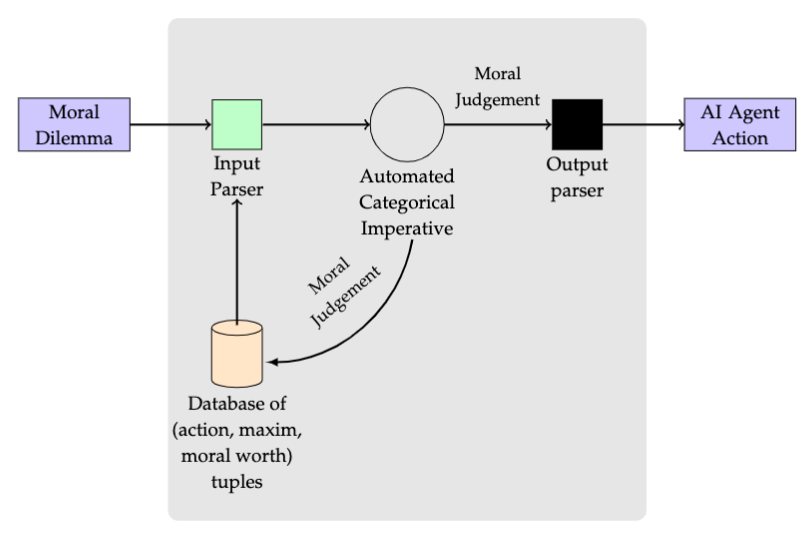
\includegraphics[scale=0.47]{inputparser.png}
\caption{A refined version of Figure \ref{fig:AIengine} in which the input parser learns from a database
of action-maxim mappings, which is in turn fed the output of my automated categorical imperative. } \label{fig:inputparser}
\end{figure}
%
\begin{isamarkuptext}%
Under Tafani's understanding of the categorical imperative, not only is automated moral reasoning
possible, but the challenge of creating an input parser or automatically formulating a maxim becomes 
easier as well. 
If the categorical imperative test is only useful to those who have some prior moral knowledge, then prior moral
knowledge can and should be used to create an input parser. Specifically, a machine learning-based approach
could learn action-maxim mappings from a database of such mappings compiled by a human being. Moreover, 
the human being could assign each maxim in the database a rightness or wrongness score. My implementation
of the automated categorical imperative would then simply check the work of this machine learning algorithm and transform
a fuzzy prediction into a provable, rigorous moral judgement. This rigorous moral judgement
could in turn be fed into the database of maxims to make the intput parser smarter. One example of 
this kind of system is shown in Figure \ref{fig:inputparser}. The combination of 
prior knowledge of some maxims' moral worth and the ability of a computer to constantly perform the
universalizability test could not only match human ethical reasoning but could perhaps surpass it
by double checking the moral intuitions that we take for granted. A computer with no common sense or prior knowledge
may be unable to reason using the categorical imperative, but one equipped with some prior knowledge
of maxims and their moral worth may even be able to reason about morality better than human beings can.%
\end{isamarkuptext}\isamarkuptrue%
%
\isadelimdocument
%
\endisadelimdocument
%
\isatagdocument
%
\isamarkupsubsection{Related Work \label{relatedwork}%
}
\isamarkuptrue%
%
\endisatagdocument
{\isafolddocument}%
%
\isadelimdocument
%
\endisadelimdocument
%
\begin{isamarkuptext}%
In 1685, Leibniz dreamed of a calculator that could resolve philosophical and theological 
disputes \citep{leibniz}. At the time, the logical and computational resources necessary to make his 
dream a reality did not exist. Today, automated ethics is a growing field, spurred in part by the 
need for ethically intelligent AI agents. Tolmeijer et al. surveyed the state of the field of 
machine ethics \citep{mesurvey} and characterized implementations in automated ethics by (1) the choice 
of ethical theory, (2) implementation design decisions (e.g. logic programming), and (3) implementation 
details (e.g. choice of logic). 

Automated ethics falls into two branches: top-down and bottom-up ethics. Top-down automated ethics begins 
with an ethical theory, whereas bottom-up automated ethics learns ethical judgements from prior 
judgements. One example of bottom-up automated ethics is Delphi, which uses deep learning to make 
ethical judgements based on a dataset of human judgements \citep{delphi}. While Delphi displays great 
flexibility, it often produces contradictory judgements, such as claiming that taxing exploitative 
profitable companies is good, but burdening successful companies with high tax rates is bad \citep{verge}. 
Because Delphi draws on error-prone human judgements instead of philosophical literature, it makes 
the same judgement errors that humans make. Moreover, because Delphi uses a bottom-up approach, 
there is no explicit ethical theory explaining its judgements, so analytically arguing for or 
against its conclusions is impossible. Top-down approaches, on the other hand, must be explicit about 
the underlying ethical theories, and are thus more explainable. 

In this paper, I use a top-down approach to formalize Kantian ethics. There is a long line of work 
automating other ethical theories, like consequentialism \citep{util1, util2} or particularism 
\citep{particularism1, particularism2}. I choose to implement Kantian ethics because, as argued in 
Section \ref{whykant}, it is the most formal and least data-intensive of the three major ethical 
traditions. Kantian ethics is a deontological, or rule based ethic, and there is prior work 
implementing other deontological theories \citep{dde, deon1, deon2}. 

Kantian ethics specifically appears to be an intuitive candidate for formalization and implementation 
and there has been both theoretical and practical work on automating Kantian ethics \citep{powers, lin}. 
In 2006, Powers argued that implementing Kantian ethics presented technical challenges, 
such as automation of a non-monotonic logic, and philosophical challenges, like a definition of the 
categorical imperative \citep{powers}. I address the former through my use of Dyadic Deontic Logic, which allows 
obligations to be retracted as context changes, and the latter through my use of the practical 
contradiction interpretation. There has also been prior work in formalizing Kantian metaphysics 
using I/O logic \citep{io}. Deontic logic, which has been implemented in Isabelle/HOL, is itself inspired 
by Kant's ``ought implies can'' principle, but it does not include a robust formalization of the entire 
categorical imperative \citep{cresswell}.

Kroy presents a formalization of the first two formulations of the categorical imperative, but wrote 
before the computational tools existed to automate such a formalization \citep{kroy}. I implement his formalization of the FUL to compare it to my system. 
Lindner and Bentzen presented one of the first implementations of a formalization of 
Kant's second formulation of the categorical imperative \citep{BL}. They present their goal as ``not to get 
close to a correct interpretation of Kant, but to show that our interpretation of Kant’s ideas can 
contribute to the development of machine ethics.'' My work builds on theirs by formalizing the 
first formulation of the categorical imperative as faithfully as possible. Staying faithful to 
philosophical literature makes my system capable of making robust and reliable judgements. 

The implementation of this paper was inspired by and builds on Benzmüller, Parent, and Farjami's 
foundational work with the LogiKEy framework for machine ethics, which includes their implementation 
of DDL in Isabelle \citep{BFP, logikey}. The LogiKEy project has been used to study metaphysics 
\citep{godel, metaphysics1}, law \citep{constitution}, and ethics \citep{gewirth}, but not 
Kant's categorical imperative.%
\end{isamarkuptext}\isamarkuptrue%
%
\isadelimdocument
%
\endisadelimdocument
%
\isatagdocument
%
\isamarkupsubsection{Conclusion%
}
\isamarkuptrue%
%
\endisatagdocument
{\isafolddocument}%
%
\isadelimdocument
%
\endisadelimdocument
%
\begin{isamarkuptext}%
In this thesis, I present a proof-of-concept implementation of automated Kantian ethics. My system
takes as input a potential action, appropriately represented, and can prove that it is obligated, 
prohibited or permissible. I represent Kant's Formula of Universal Law in a deontic logic and 
implement this logic in the Isabelle/HOL interactive theorem prover, which can automatically prove or 
refute theorems in my custom logic. I also contribute a testing framework that demonstrates that
my implementation of Kantian ethics is more faithful to philosophical literature than two other 
potential implementations. My completed system can, when given appropriate factual background, make
philosophically mature judgements about complex moral dilemmas. This work is one step towards building 
morally sophisticated artifical agents.

The idea of fully automated artificial agents navigating the world without human supervision
may be terrifying, but progress in AI indicates that such a future is likely closer than we think. 
Philosophers, regulators, and computer scientists are sounding the alarm about the dangers of developing
this kind of AI. Insofar as developers will continue to ignore these warnings and develop increasingly 
independent AI, there is a dire need to program such AI with some notion of ethics. If AI is navigating
human society, then it is making ethically-tinged decisions at all times. Ethics is inescapable; 
if AI developers and computer scientists ignore it, then they will be building machines that make decisions
based on some set of unknown, implicit ethical values. Countless examples, from the Alleghany family services screening
algorithm that is biased against poor families to search algorithms that associate black-sounding names
with crime, demonstrate that such implicit ethics usually codifies the biases, prejudices, and moral
failings of the society in which it is developed \citep{eubanks, sweeney}. AI will inevitably make judgements on moral dilemmas, 
and automated ethics is necessary to make these judgements morally correct. 

Given that the discpline of philosophy has spent centuries debating such judgements and their theoretical 
underpinnings, such AI will be most trustworthy, nuanced, consistent, and mature when it is faithful to 
philosophical literature. In order to develop high-quality automated ethics, computer scientists and 
philosophers must work together. This thesis is an experiment in marrying philosophy and computer science 
to create automated ethics that is both technically and philosophically advanced. Neither discipline alone
can address the pressing need for ethical AI.

This work is an early proof-of-concept. It demonstrates the potential of top-down, logic programming 
approaches to automated ethics and shows that it is possible to faithfully automate an ethical theory as
complex as Kantian ethics. There are open questions that must be resolved before a system like this 
could be used in practice, but this project demonstrates that these questions are within closer reach
than they may seem. Automated ethics does not need to limit itself to simple, flattened versions of 
ethical theories. With technical and philosophical progress, faithful automated ethics is possible.
Growing public consciousness about the dangers of unregulated AI is creating momentum in machine ethics; 
work like Delphi demonstrates that the time is ripe to create usable, reliable automated ethics. This 
thesis is one step towards building computers that can think ethically in the richest sense of the word.%
\end{isamarkuptext}\isamarkuptrue%
%
\isadelimtheory
%
\endisadelimtheory
%
\isatagtheory
%
\endisatagtheory
{\isafoldtheory}%
%
\isadelimtheory
%
\endisadelimtheory
%
\end{isabellebody}%
\endinput
%:%file=~/Desktop/cs91r/paper/thesis_5_discussion.thy%:%
%:%24=6%:%
%:%28=8%:%
%:%39=11%:%
%:%40=12%:%
%:%41=13%:%
%:%42=14%:%
%:%43=15%:%
%:%44=16%:%
%:%45=17%:%
%:%46=18%:%
%:%47=19%:%
%:%50=21%:%
%:%51=22%:%
%:%52=23%:%
%:%53=24%:%
%:%54=25%:%
%:%55=26%:%
%:%56=27%:%
%:%57=28%:%
%:%58=29%:%
%:%59=30%:%
%:%60=31%:%
%:%61=32%:%
%:%62=33%:%
%:%63=34%:%
%:%64=35%:%
%:%65=36%:%
%:%66=37%:%
%:%67=38%:%
%:%68=39%:%
%:%69=40%:%
%:%70=41%:%
%:%71=42%:%
%:%72=43%:%
%:%73=44%:%
%:%74=45%:%
%:%75=46%:%
%:%76=47%:%
%:%77=48%:%
%:%78=49%:%
%:%79=50%:%
%:%80=51%:%
%:%81=52%:%
%:%82=53%:%
%:%83=54%:%
%:%84=55%:%
%:%85=56%:%
%:%86=57%:%
%:%87=58%:%
%:%88=59%:%
%:%89=60%:%
%:%90=61%:%
%:%91=62%:%
%:%92=63%:%
%:%93=64%:%
%:%94=65%:%
%:%95=66%:%
%:%96=67%:%
%:%97=68%:%
%:%98=69%:%
%:%99=70%:%
%:%100=71%:%
%:%101=72%:%
%:%102=73%:%
%:%103=74%:%
%:%104=75%:%
%:%105=76%:%
%:%106=77%:%
%:%107=78%:%
%:%108=79%:%
%:%109=80%:%
%:%110=81%:%
%:%111=82%:%
%:%112=83%:%
%:%113=84%:%
%:%114=85%:%
%:%115=86%:%
%:%116=87%:%
%:%117=88%:%
%:%118=89%:%
%:%119=90%:%
%:%120=91%:%
%:%121=92%:%
%:%122=93%:%
%:%123=94%:%
%:%124=95%:%
%:%125=96%:%
%:%126=97%:%
%:%127=98%:%
%:%128=99%:%
%:%129=100%:%
%:%130=101%:%
%:%131=102%:%
%:%132=103%:%
%:%133=104%:%
%:%134=105%:%
%:%135=106%:%
%:%136=107%:%
%:%137=108%:%
%:%138=109%:%
%:%139=110%:%
%:%140=111%:%
%:%141=112%:%
%:%142=113%:%
%:%143=114%:%
%:%144=115%:%
%:%145=116%:%
%:%146=117%:%
%:%147=118%:%
%:%148=119%:%
%:%149=120%:%
%:%150=121%:%
%:%151=122%:%
%:%152=123%:%
%:%153=124%:%
%:%154=125%:%
%:%155=126%:%
%:%156=127%:%
%:%157=128%:%
%:%158=129%:%
%:%159=130%:%
%:%160=131%:%
%:%161=132%:%
%:%162=133%:%
%:%163=134%:%
%:%164=135%:%
%:%165=136%:%
%:%166=137%:%
%:%167=138%:%
%:%168=139%:%
%:%169=140%:%
%:%170=141%:%
%:%171=142%:%
%:%180=144%:%
%:%192=146%:%
%:%193=147%:%
%:%194=148%:%
%:%195=149%:%
%:%196=150%:%
%:%197=151%:%
%:%198=152%:%
%:%199=153%:%
%:%200=154%:%
%:%201=155%:%
%:%202=156%:%
%:%211=158%:%
%:%223=160%:%
%:%224=161%:%
%:%225=162%:%
%:%226=163%:%
%:%227=164%:%
%:%228=165%:%
%:%229=166%:%
%:%230=167%:%
%:%231=168%:%
%:%232=169%:%
%:%233=170%:%
%:%234=171%:%
%:%235=172%:%
%:%236=173%:%
%:%237=174%:%
%:%238=175%:%
%:%239=176%:%
%:%240=177%:%
%:%241=178%:%
%:%242=179%:%
%:%243=180%:%
%:%244=181%:%
%:%245=182%:%
%:%246=183%:%
%:%247=184%:%
%:%248=185%:%
%:%249=186%:%
%:%250=187%:%
%:%251=188%:%
%:%252=189%:%
%:%253=190%:%
%:%254=191%:%
%:%255=192%:%
%:%256=193%:%
%:%257=194%:%
%:%258=195%:%
%:%259=196%:%
%:%260=197%:%
%:%261=198%:%
%:%262=199%:%
%:%263=200%:%
%:%264=201%:%
%:%265=202%:%
%:%266=203%:%
%:%267=204%:%
%:%268=205%:%
%:%269=206%:%
%:%270=207%:%
%:%271=208%:%
%:%272=209%:%
%:%273=210%:%
%:%274=211%:%
%:%275=212%:%
%:%276=213%:%
%:%277=214%:%
%:%278=215%:%
%:%279=216%:%
%:%280=217%:%
%:%281=218%:%
%:%282=219%:%
%:%283=220%:%
%:%284=221%:%
%:%285=222%:%
%:%286=223%:%
%:%287=224%:%
%:%288=225%:%
%:%289=226%:%
%:%290=227%:%
%:%291=228%:%
%:%292=229%:%
%:%293=230%:%
%:%294=231%:%
%:%295=232%:%
%:%296=233%:%
%:%297=234%:%
%:%298=235%:%
%:%299=236%:%
%:%300=237%:%
%:%301=238%:%
%:%302=239%:%
%:%303=240%:%
%:%304=241%:%
%:%305=242%:%
%:%306=243%:%
%:%307=244%:%
%:%308=245%:%
%:%309=246%:%
%:%310=247%:%
%:%311=248%:%
%:%312=249%:%
%:%313=250%:%
%:%314=251%:%
%:%315=252%:%
%:%316=253%:%
%:%317=254%:%
%:%318=255%:%
%:%319=256%:%
%:%320=257%:%
%:%321=258%:%
%:%322=259%:%
%:%323=260%:%
%:%324=261%:%
%:%325=262%:%
%:%326=263%:%
%:%327=264%:%
%:%328=265%:%
%:%329=266%:%
%:%330=267%:%
%:%331=268%:%
%:%332=269%:%
%:%333=270%:%
%:%334=271%:%
%:%335=272%:%
%:%336=273%:%
%:%337=274%:%
%:%338=275%:%
%:%339=276%:%
%:%340=277%:%
%:%341=278%:%
%:%342=279%:%
%:%343=280%:%
%:%344=281%:%
%:%345=282%:%
%:%346=283%:%
%:%347=284%:%
%:%348=285%:%
%:%349=286%:%
%:%350=287%:%
%:%351=288%:%
%:%352=289%:%
%:%353=290%:%
%:%354=291%:%
%:%355=292%:%
%:%356=293%:%
%:%357=294%:%
%:%358=295%:%
%:%359=296%:%
%:%360=297%:%
%:%361=298%:%
%:%362=299%:%
%:%363=300%:%
%:%364=301%:%
%:%365=302%:%
%:%366=303%:%
%:%367=304%:%
%:%368=305%:%
%:%369=306%:%
%:%370=307%:%
%:%371=308%:%
%:%372=309%:%
%:%373=310%:%
%:%374=311%:%
%:%375=312%:%
%:%376=313%:%
%:%377=314%:%
%:%378=315%:%
%:%379=316%:%
%:%380=317%:%
%:%381=318%:%
%:%382=319%:%
%:%383=320%:%
%:%384=321%:%
%:%385=322%:%
%:%386=323%:%
%:%387=324%:%
%:%388=325%:%
%:%389=326%:%
%:%390=327%:%
%:%391=328%:%
%:%392=329%:%
%:%393=330%:%
%:%394=331%:%
%:%395=332%:%
%:%396=333%:%
%:%397=334%:%
%:%398=335%:%
%:%399=336%:%
%:%400=337%:%
%:%401=338%:%
%:%402=339%:%
%:%403=340%:%
%:%404=341%:%
%:%405=342%:%
%:%406=343%:%
%:%407=344%:%
%:%408=345%:%
%:%409=346%:%
%:%410=347%:%
%:%411=348%:%
%:%412=349%:%
%:%413=350%:%
%:%414=351%:%
%:%415=352%:%
%:%416=353%:%
%:%425=356%:%
%:%437=358%:%
%:%438=359%:%
%:%439=360%:%
%:%440=361%:%
%:%441=362%:%
%:%442=363%:%
%:%443=364%:%
%:%444=365%:%
%:%445=366%:%
%:%446=367%:%
%:%447=368%:%
%:%448=369%:%
%:%449=370%:%
%:%450=371%:%
%:%451=372%:%
%:%452=373%:%
%:%453=374%:%
%:%454=375%:%
%:%455=376%:%
%:%456=377%:%
%:%457=378%:%
%:%458=379%:%
%:%459=380%:%
%:%460=381%:%
%:%461=382%:%
%:%462=383%:%
%:%463=384%:%
%:%464=385%:%
%:%465=386%:%
%:%466=387%:%
%:%467=388%:%
%:%468=389%:%
%:%469=390%:%
%:%470=391%:%
%:%471=392%:%
%:%472=393%:%
%:%473=394%:%
%:%474=395%:%
%:%475=396%:%
%:%476=397%:%
%:%477=398%:%
%:%478=399%:%
%:%479=400%:%
%:%480=401%:%
%:%481=402%:%
%:%482=403%:%
%:%483=404%:%
%:%484=405%:%
%:%485=406%:%
%:%486=407%:%
%:%487=408%:%
%:%488=409%:%
%:%489=410%:%
%:%490=411%:%
%:%491=412%:%
%:%492=413%:%
%:%493=414%:%
%:%494=415%:%
%:%495=416%:%
%:%496=417%:%
%:%497=418%:%
%:%498=419%:%
%:%499=420%:%
%:%500=421%:%
%:%501=422%:%
%:%502=423%:%
%:%503=424%:%
%:%512=426%:%
%:%524=428%:%
%:%525=429%:%
%:%526=430%:%
%:%527=431%:%
%:%528=432%:%
%:%529=433%:%
%:%530=434%:%
%:%531=435%:%
%:%532=436%:%
%:%533=437%:%
%:%534=438%:%
%:%535=439%:%
%:%536=440%:%
%:%537=441%:%
%:%538=442%:%
%:%539=443%:%
%:%540=444%:%
%:%541=445%:%
%:%542=446%:%
%:%543=447%:%
%:%544=448%:%
%:%545=449%:%
%:%546=450%:%
%:%547=451%:%
%:%548=452%:%
%:%549=453%:%
%:%550=454%:%
%:%551=455%:%
%:%552=456%:%
%:%553=457%:%
%:%554=458%:%
%:%555=459%:%
%:%556=460%:%
%:%557=461%:%
%:%558=462%:%
%:%559=463%:%
%:%560=464%:%
%:%561=465%:%
%:%562=466%:%
%:%563=467%:%
%:%564=468%:%
%:%565=469%:%
%:%566=470%:%
%:%567=471%:%
%:%568=472%:%
%:%569=473%:%
%:%570=474%:%
%:%571=475%:%
%:%572=476%:%
%:%573=477%:%
%:%574=478%:%
%:%575=479%:%
%:%576=480%:%
%:%577=481%:%
%:%578=482%:%
%:%579=483%:%
%:%580=484%:%
%:%581=485%:%
%:%582=486%:%
%:%583=487%:%
%:%584=488%:%
%:%585=489%:%
%:%586=490%:%
%:%587=491%:%
%:%588=492%:%
%:%589=493%:%
%:%590=494%:%
%:%591=495%:%
%:%592=496%:%
%:%593=497%:%
%:%594=498%:%
%:%595=499%:%
%:%596=500%:%
%:%597=501%:%
%:%598=502%:%
%:%599=503%:%
%:%600=504%:%
%:%601=505%:%
%:%602=506%:%
%:%603=507%:%
%:%612=510%:%
%:%624=513%:%
%:%625=514%:%
%:%626=515%:%
%:%627=516%:%
%:%628=517%:%
%:%629=518%:%
%:%630=519%:%
%:%631=520%:%
%:%632=521%:%
%:%633=522%:%
%:%634=523%:%
%:%635=524%:%
%:%636=525%:%
%:%637=526%:%
%:%638=527%:%
%:%639=528%:%
%:%640=529%:%
%:%641=530%:%
%:%642=531%:%
%:%643=532%:%
%:%644=533%:%
%:%645=534%:%
%:%646=535%:%
%:%647=536%:%
%:%648=537%:%
%:%649=538%:%
%:%650=539%:%
%:%651=540%:%
%:%652=541%:%
%:%653=542%:%
%:%654=543%:%
%:%655=544%:%
%:%656=545%:%
%:%657=546%:%
%:%658=547%:%
%:%659=548%:%
%:%660=549%:%
%:%661=550%:%
%:%662=551%:%
%:%663=552%:%
%:%664=553%:%
%:%665=554%:%
%:%666=555%:%
%:%667=556%:%
%:%668=557%:%
%:%669=558%:%
%:%670=559%:%
%:%671=560%:%
%:%672=561%:%
%:%673=562%:%
%:%674=563%:%
%:%675=564%:%
%:%676=565%:%
%:%677=566%:%
%:%678=567%:%
%:%679=568%:%
%:%680=569%:%
%:%681=570%:%
%:%682=571%:%
%:%683=572%:%
%:%684=573%:%
%:%685=574%:%
%:%686=575%:%
%:%687=576%:%
%:%688=577%:%
%:%689=578%:%
%:%690=579%:%
%:%691=580%:%
%:%692=581%:%
%:%693=582%:%
%:%694=583%:%
%:%695=584%:%
%:%696=585%:%
%:%697=586%:%
%:%698=587%:%
%:%699=588%:%
%:%700=589%:%
%:%701=590%:%
%:%702=591%:%
%:%703=592%:%
%:%704=593%:%
%:%705=594%:%
%:%706=595%:%
%:%707=596%:%
%:%708=597%:%
%:%709=598%:%
%:%710=599%:%
%:%711=600%:%
%:%712=601%:%
%:%713=602%:%
%:%714=603%:%
%:%715=604%:%
%:%716=605%:%
%:%717=606%:%
%:%718=607%:%
%:%719=608%:%
%:%720=609%:%
%:%721=610%:%
%:%722=611%:%
%:%723=612%:%
%:%724=613%:%
%:%725=614%:%
%:%726=615%:%
%:%727=616%:%
%:%728=617%:%
%:%729=618%:%
%:%730=619%:%
%:%731=620%:%
%:%732=621%:%
%:%733=622%:%
%:%734=623%:%
%:%735=624%:%
%:%736=625%:%
%:%737=626%:%
%:%738=627%:%
%:%739=628%:%
%:%740=629%:%
%:%741=630%:%
%:%742=631%:%
%:%745=633%:%
%:%746=634%:%
%:%747=635%:%
%:%748=636%:%
%:%749=637%:%
%:%750=638%:%
%:%753=639%:%
%:%754=640%:%
%:%755=641%:%
%:%756=642%:%
%:%757=643%:%
%:%758=644%:%
%:%759=645%:%
%:%760=646%:%
%:%761=647%:%
%:%762=648%:%
%:%763=649%:%
%:%764=650%:%
%:%765=651%:%
%:%766=652%:%
%:%767=653%:%
%:%768=654%:%
%:%777=658%:%
%:%789=660%:%
%:%790=661%:%
%:%791=662%:%
%:%792=663%:%
%:%793=664%:%
%:%794=665%:%
%:%795=666%:%
%:%796=667%:%
%:%797=668%:%
%:%798=669%:%
%:%799=670%:%
%:%800=671%:%
%:%801=672%:%
%:%802=673%:%
%:%803=674%:%
%:%804=675%:%
%:%805=676%:%
%:%806=677%:%
%:%807=678%:%
%:%808=679%:%
%:%809=680%:%
%:%810=681%:%
%:%811=682%:%
%:%812=683%:%
%:%813=684%:%
%:%814=685%:%
%:%815=686%:%
%:%816=687%:%
%:%817=688%:%
%:%818=689%:%
%:%819=690%:%
%:%820=691%:%
%:%821=692%:%
%:%822=693%:%
%:%823=694%:%
%:%824=695%:%
%:%825=696%:%
%:%826=697%:%
%:%827=698%:%
%:%828=699%:%
%:%829=700%:%
%:%830=701%:%
%:%831=702%:%
%:%832=703%:%
%:%833=704%:%
%:%834=705%:%
%:%835=706%:%
%:%836=707%:%
%:%837=708%:%
%:%838=709%:%
%:%839=710%:%
%:%840=711%:%
%:%849=713%:%
%:%861=715%:%
%:%862=716%:%
%:%863=717%:%
%:%864=718%:%
%:%865=719%:%
%:%866=720%:%
%:%867=721%:%
%:%868=722%:%
%:%869=723%:%
%:%870=724%:%
%:%871=725%:%
%:%872=726%:%
%:%873=727%:%
%:%874=728%:%
%:%875=729%:%
%:%876=730%:%
%:%877=731%:%
%:%878=732%:%
%:%879=733%:%
%:%880=734%:%
%:%881=735%:%
%:%882=736%:%
%:%883=737%:%
%:%884=738%:%
%:%885=739%:%
%:%886=740%:%
%:%887=741%:%
%:%888=742%:%
%:%889=743%:%
%:%890=744%:%
%:%891=745%:%
%:%892=746%:%
%:%893=747%:%
%:%894=748%:%
%:%895=749%:%
%:%896=750%:%
%:%897=751%:%
%:%898=752%:%
%:%899=753%:%